\chapter{Evaluation}
\label{chap:evaluation}
\section{Test Environment}
The measurements were recorded in the University of Miskolc's Institution of Information Science, Department of Information Technology. The recorded values were taken with 4 identical smart phones with Android operating system. Two of the tests were recorded without any disturbance, just the natural reflective surfaces in the room, and two were recorded with people present in the room. The latest showed a lot of inconsistencies on the recorded values, further increasing the need for a filter on the preprocessed data. As noise grows, the filters value increases, as it can be smoothed out the naturally occurring  jumps on the diagram.
The following sample is taken from the data set used to test the filters on:
\begin{figure}[h!]
\begin{verbatim}
Time,SSID,MAC,Signal
2016/02/02.09:43:33,IITAP1,E0:5F:B9:0C:71:27,-39
2016/02/02.09:43:33,IITAP1-GUEST,E2:5F:B9:0C:71:27,-39
2016/02/02.09:43:33,KRZ,0:18:E7:DE:A3:90,-48
2016/02/02.09:43:33,LABOR,00:14:C1:33:A0:78,-72
2016/02/02.09:43:33,GEIAKFSZ,F8:66:F2:AD:E6:91,-76
2016/02/02.09:43:33,doa207,14:CC:20:57:3D:0C,-67
2016/02/02.09:43:33,dd,00:19:E0:65:E4:F2,-84
2016/02/02.09:43:33,doa208,F8:66:F2:AD:E6:79,-81
2016/02/02.09:43:35,IITAP1,E0:5F:B9:0C:71:27,-40

\end{verbatim}
\caption{Data set sample}
\label{fig:Datasample}
\end{figure}

\section{Comparison}
The filters have clearly shown that their usage have increased the accuracy and steadiness of the WiFi signals. These results mean that the usage of preprocessing filters can be used to steadily improve positioning.
The comparison of the diagrams
\begin{figure}[h!]
	\centering
		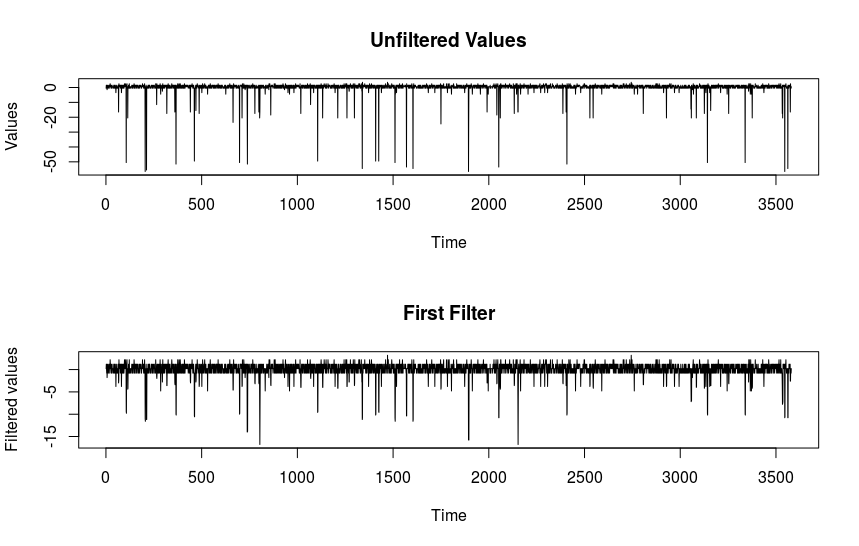
\includegraphics[width=.9\linewidth]{figures/comp1.png}
		\caption{Comparison of the values of the raw and the values after first filter
		}\label{fig:firstComp}
\end{figure}


As seen on the Figure \ref{fig:firstComp} the filter marginally increases the continuity of the series.
It dynamically reduces the range of numbers in which the series works in. Please note that the original, unfiltered series' lowest value was exceeded -50, where with the first filter it only goes down to around -15.


\begin{figure}[h!]
	\centering
		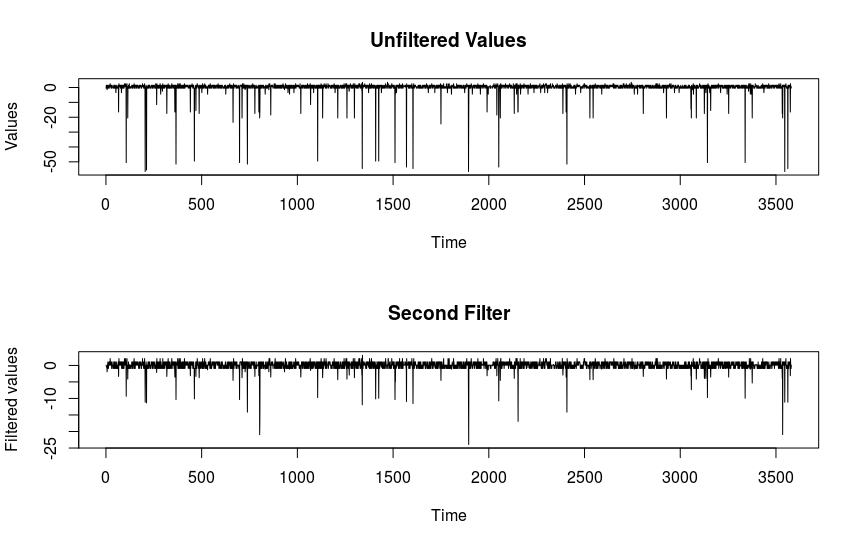
\includegraphics[width=.9\linewidth]{figures/comp2.png}
		\caption{Comparison of the values of the raw and the values after second filter }\label{fig:secondComp}
\end{figure}

The second filter as seen on Figure \ref{fig:secondComp} is similar in nature. It reduces the range of numbers by more then half of the original values. It has a more complex algorithm, but it is less effective than the more simple, first filter, where the threshold isn't computed dynamically. It may be more useful in environments where filtering has to be done on unknown data sets.	

\begin{figure}[h!]
	\centering
		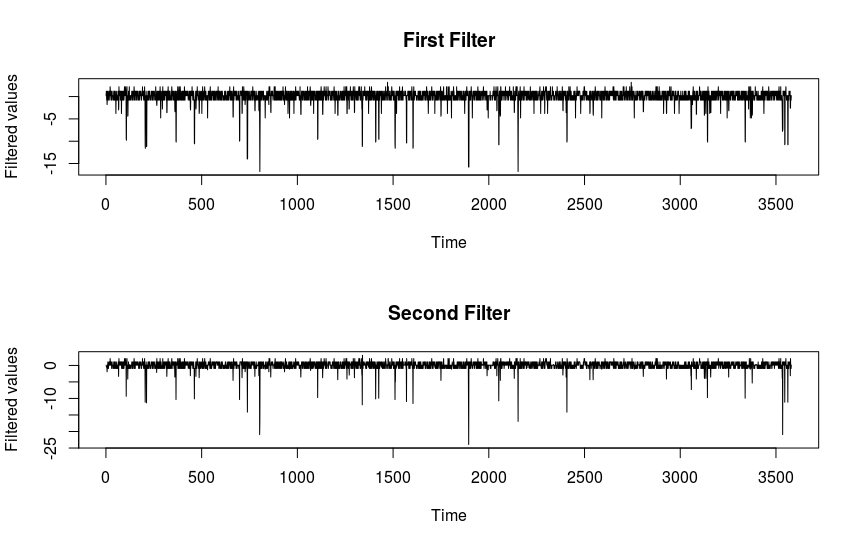
\includegraphics[width=.9\linewidth]{figures/comp3.png}
		\caption{Comparison of the values of the two filters 
		}\label{fig:thirdComp}
\end{figure}


\section{Suggestion} 
The first filter works well if you can specify the threshold amount well. It can marginally reduce the range, thus increasing the efficiency and accuracy of WiFi RSSI measurement in an indoor positioning environment.  The second filter is more dynamic in nature, as it can work on any data set without setting a certain threshold. Although less effective, it may be more practical to use in real life situations. More filters can be developed in the future to increase effectiveness. Computational complexity also has to be taken in mind. The first and second algorithm are quite simple, and could be run on most devices, but as effectiveness grows, so could complexity, rendering more and more devices unable to use preprocessing filters.
